\documentclass[12pt,oneside,english,a4paper]{article}
\usepackage{babel}
\usepackage[utf8]{inputenc}
\usepackage[T1]{fontenc}
\usepackage{color}
\usepackage{graphicx}
\usepackage{wallpaper}
\usepackage{wrapfig,booktabs}

\usepackage{fancyhdr}

\usepackage{fourier-orns}
\newcommand{\dash}{\noindent \newline\textcolor{black}{\hrulefill~ \raisebox{-2.5pt}[10pt][10pt]{\leafright \decofourleft \decothreeleft  \aldineright \decotwo \floweroneleft \decoone   \floweroneright \decotwo \aldineleft\decothreeright \decofourright \leafleft} ~  \hrulefill}}

\usepackage{titlesec}
\titleformat*{\section}{\it\huge\bfseries}
\titleformat*{\subsection}{\it\huge\bfseries}
\titleformat*{\subsubsection}{\it\LARGE\bfseries}
\titleformat*{\paragraph}{\huge\bfseries}
\titleformat*{\subparagraph}{\LARGE\bfseries}

\usepackage[left=20px,right=20px,top=50px,bottom=50px,paperwidth=8in,paperheight=12in]{geometry}

\usepackage[cjk]{kotex}
\usepackage{amsthm} 
\usepackage{amsmath} 
\usepackage{amsfonts}
\usepackage{enumerate} 
\usepackage{cite}
\usepackage{graphics} 
\usepackage{graphicx,lscape} 
\usepackage{subcaption}
\usepackage{algpseudocode}
\usepackage{algorithm}
\usepackage{titlesec}
\usepackage{cite, url}
\usepackage{amssymb}

\def\bk{\paragraph{\Large$$}\Large}
\def\ck{\paragraph{\Large$\bullet$}\Large}
\def\sol{\paragraph{\Large(sol)}\Large}
\def\pf{\paragraph{\Large(pf)}\Large}
\def\note{\paragraph{\Large\textit{\underline{note:}}}\Large}
\def\ex{\paragraph{\Large\textit{example:}}\Large}
\newcommand{\para}[1]{\paragraph{\Large\it\underline{\textbf{#1:}}}\Large}
\newcommand{\parablue}[1]{\paragraph{\Large\textcolor{blue}{\it\underline{\textbf{#1:}}}}\Large}
\newcommand{\parared}[1]{\paragraph{\Large\textcolor{red}{\it\underline{\textbf{#1:}}}}\Large}


\def\one{\paragraph{\Large(1)}\Large}
\def\two{\paragraph{\Large(2)}\Large}
\def\three{\paragraph{\Large(3)}\Large}
\def\four{\paragraph{\Large(4)}\Large}
\def\five{\paragraph{\Large(5)}\Large}
\def\six{\paragraph{\Large(6)}\Large}
\def\seven{\paragraph{\Large(7)}\Large}
\def\eight{\paragraph{\Large(8)}\Large}
\def\nine{\paragraph{\Large(9)}\Large}
\def\ten{\paragraph{\Large(10)}\Large}

\def\cka{\paragraph{\Large(a)}\Large}
\def\ckb{\paragraph{\Large(b)}\Large}
\def\ckc{\paragraph{\Large(c)}\Large}
\def\ckd{\paragraph{\Large(d)}\Large}
\def\cke{\paragraph{\Large(e)}\Large}
\def\ckf{\paragraph{\Large(f)}\Large}
\def\ckg{\paragraph{\Large(g)}\Large}
\def\ckh{\paragraph{\Large(h)}\Large}
\def\cki{\paragraph{\Large(i)}\Large}
\def\ckj{\paragraph{\Large(j)}\Large}

\newcommand{\bs}[1]{\mbox{\boldmath $#1$}}

\newcommand{\bsa}{\mbox{\boldmath $a$}}
\newcommand{\bsb}{\mbox{\boldmath $b$}}
\newcommand{\bsc}{\mbox{\boldmath $c$}}
\newcommand{\bsd}{\mbox{\boldmath $d$}}
\newcommand{\bse}{\mbox{\boldmath $e$}}
\newcommand{\bsf}{\mbox{\boldmath $f$}}
\newcommand{\bsg}{\mbox{\boldmath $g$}}
\newcommand{\bsh}{\mbox{\boldmath $h$}}
\newcommand{\bsi}{\mbox{\boldmath $i$}}
\newcommand{\bsj}{\mbox{\boldmath $j$}}
\newcommand{\bsk}{\mbox{\boldmath $k$}}
\newcommand{\bsl}{\mbox{\boldmath $l$}}
\newcommand{\bsm}{\mbox{\boldmath $m$}}
\newcommand{\bsn}{\mbox{\boldmath $n$}}
\newcommand{\bso}{\mbox{\boldmath $o$}}
\newcommand{\bsp}{\mbox{\boldmath $p$}}
\newcommand{\bsq}{\mbox{\boldmath $q$}}
\newcommand{\bsr}{\mbox{\boldmath $r$}}
\newcommand{\bss}{\mbox{\boldmath $s$}}
\newcommand{\bst}{\mbox{\boldmath $t$}}
\newcommand{\bsu}{\mbox{\boldmath $u$}}
\newcommand{\bsv}{\mbox{\boldmath $v$}}
\newcommand{\bsw}{\mbox{\boldmath $w$}}
\newcommand{\bsx}{\mbox{\boldmath $x$}}
\newcommand{\bsy}{\mbox{\boldmath $y$}}
\newcommand{\bsz}{\mbox{\boldmath $z$}}

\newcommand{\bfa}{\mbox{$\bf{a}$}}
\newcommand{\bfb}{\mbox{$\bf{b}$}}
\newcommand{\bfc}{\mbox{$\bf{c}$}}
\newcommand{\bfd}{\mbox{$\bf{d}$}}
\newcommand{\bfe}{\mbox{$\bf{e}$}}
\newcommand{\bff}{\mbox{$\bf{f}$}}
\newcommand{\bfg}{\mbox{$\bf{g}$}}
\newcommand{\bfh}{\mbox{$\bf{h}$}}
\newcommand{\bfi}{\mbox{$\bf{i}$}}
\newcommand{\bfj}{\mbox{$\bf{j}$}}
\newcommand{\bfk}{\mbox{$\bf{k}$}}
\newcommand{\bfl}{\mbox{$\bf{l}$}}
\newcommand{\bfm}{\mbox{$\bf{m}$}}
\newcommand{\bfn}{\mbox{$\bf{n}$}}
\newcommand{\bfo}{\mbox{$\bf{o}$}}
\newcommand{\bfp}{\mbox{$\bf{p}$}}
\newcommand{\bfq}{\mbox{$\bf{q}$}}
\newcommand{\bfr}{\mbox{$\bf{r}$}}
\newcommand{\bfs}{\mbox{$\bf{s}$}}
\newcommand{\bft}{\mbox{$\bf{t}$}}
\newcommand{\bfu}{\mbox{$\bf{u}$}}
\newcommand{\bfv}{\mbox{$\bf{v}$}}
\newcommand{\bfw}{\mbox{$\bf{w}$}}
\newcommand{\bfx}{\mbox{$\bf{x}$}}
\newcommand{\bfy}{\mbox{$\bf{y}$}}
\newcommand{\bfz}{\mbox{$\bf{z}$}}

\newcommand{\bsA}{\mbox{\boldmath $A$}}
\newcommand{\bsB}{\mbox{\boldmath $B$}}
\newcommand{\bsC}{\mbox{\boldmath $C$}}
\newcommand{\bsD}{\mbox{\boldmath $D$}}
\newcommand{\bsE}{\mbox{\boldmath $E$}}
\newcommand{\bsF}{\mbox{\boldmath $F$}}
\newcommand{\bsG}{\mbox{\boldmath $G$}}
\newcommand{\bsH}{\mbox{\boldmath $H$}}
\newcommand{\bsI}{\mbox{\boldmath $I$}}
\newcommand{\bsJ}{\mbox{\boldmath $J$}}
\newcommand{\bsK}{\mbox{\boldmath $K$}}
\newcommand{\bsL}{\mbox{\boldmath $L$}}
\newcommand{\bsM}{\mbox{\boldmath $M$}}
\newcommand{\bsN}{\mbox{\boldmath $N$}}
\newcommand{\bsO}{\mbox{\boldmath $O$}}
\newcommand{\bsP}{\mbox{\boldmath $P$}}
\newcommand{\bsQ}{\mbox{\boldmath $Q$}}
\newcommand{\bsR}{\mbox{\boldmath $R$}}
\newcommand{\bsS}{\mbox{\boldmath $S$}}
\newcommand{\bsT}{\mbox{\boldmath $T$}}
\newcommand{\bsU}{\mbox{\boldmath $U$}}
\newcommand{\bsV}{\mbox{\boldmath $V$}}
\newcommand{\bsW}{\mbox{\boldmath $W$}}
\newcommand{\bsX}{\mbox{\boldmath $X$}}
\newcommand{\bsY}{\mbox{\boldmath $Y$}}
\newcommand{\bsZ}{\mbox{\boldmath $Z$}}

\newcommand{\bfA}{\mbox{$\bf{A}$}}
\newcommand{\bfB}{\mbox{$\bf{B}$}}
\newcommand{\bfC}{\mbox{$\bf{C}$}}
\newcommand{\bfD}{\mbox{$\bf{D}$}}
\newcommand{\bfE}{\mbox{$\bf{E}$}}
\newcommand{\bfF}{\mbox{$\bf{F}$}}
\newcommand{\bfG}{\mbox{$\bf{G}$}}
\newcommand{\bfH}{\mbox{$\bf{H}$}}
\newcommand{\bfI}{\mbox{$\bf{I}$}}
\newcommand{\bfJ}{\mbox{$\bf{J}$}}
\newcommand{\bfK}{\mbox{$\bf{K}$}}
\newcommand{\bfL}{\mbox{$\bf{L}$}}
\newcommand{\bfM}{\mbox{$\bf{M}$}}
\newcommand{\bfN}{\mbox{$\bf{N}$}}
\newcommand{\bfO}{\mbox{$\bf{O}$}}
\newcommand{\bfP}{\mbox{$\bf{P}$}}
\newcommand{\bfQ}{\mbox{$\bf{Q}$}}
\newcommand{\bfR}{\mbox{$\bf{R}$}}
\newcommand{\bfS}{\mbox{$\bf{S}$}}
\newcommand{\bfT}{\mbox{$\bf{T}$}}
\newcommand{\bfU}{\mbox{$\bf{U}$}}
\newcommand{\bfV}{\mbox{$\bf{V}$}}
\newcommand{\bfW}{\mbox{$\bf{W}$}}
\newcommand{\bfX}{\mbox{$\bf{X}$}}
\newcommand{\bfY}{\mbox{$\bf{Y}$}}
\newcommand{\bfZ}{\mbox{$\bf{Z}$}}

\DeclareMathOperator*{\argmin}{argmin} 
\DeclareMathOperator*{\argmax}{argmax} 

\usepackage[svgnames]{xcolor}
\usepackage{listings}

\lstset{language=R,
    basicstyle=\Large\tt,
    stringstyle=\color{DarkGreen},
    otherkeywords={0,1,2,3,4,5,6,7,8,9},
    morekeywords={TRUE,FALSE},
    deletekeywords={data,frame,length,as,character},
    %keywordstyle=\color{blue},
    commentstyle=\color{DarkGreen},
}

\CJKscale{0.9}
\begin{document}

\section{암기요소}

\subsection{some useful equation}
\ck ($\pi$가 \emph{given}일때) $v_{\pi}(s)$의 벨만방정식.
\begin{align*}
v_{\pi}(s)=\sum_{a}\pi(a|s)\sum_{s',r}p(s',r|s,a)\Big[r+\gamma v_{\pi}(s')\Big] 
\end{align*}
\note 여기에서 $v_{\pi}(s)$는 $\pi$가 바뀌면 변화한다. 
\note 결국 
\[
v_{\pi}(s)=\mathbb{E}_{\pi,a}r(s,a)
\]

\section{Finite MDP}
\ck 설명의 편의를 위해서 아래그림과 같이 $4\times 4$개의 격자가 있는 세계에서 로봇이 움직이는 일반적인 예제를 특정하자. 음영처리된 부분에 도착하면 로봇이 더이상 움직이지 않는다고 가정하자. 참고로 이렇게 일정한 시간이 지나면 언제가 끝이나는 task 를 \textbf{에피소드-태스크}라고 한다. 이 예제를 포함하여 바둑이나 장기와 같은것도 일정한 시간이 지나면 언젠가 끝나기 때문에 \textbf{에피소드-테스크}의 한 예이다. 반대로 시간이 지나도 끝나지 않는 task 를 \textbf{컨티뉴잉-태스크}라고 한다.
\begin{figure}[h]
\center
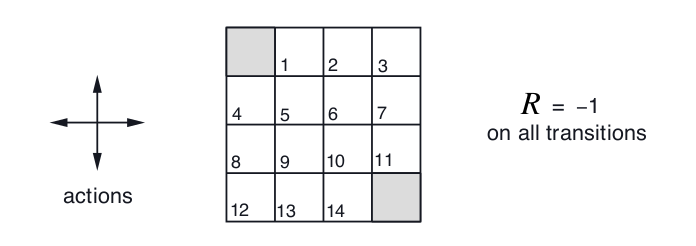
\includegraphics[width=1\textwidth]{Fig4-1.png}
\caption{셔튼교재 P.92, terminal state로 가기전까지 계속 음의 보상값 $-1$을 받는다. }
\end{figure}

\parablue{state} $4\times 4$ 격자위에서 로봇이 움직이고 있으므로 로봇이 존재할 수 있는 all possible states 는 총 16개이다. 여기에서 음영처리된 부분에 로봇이 도착하면 task가 종료되는데 이런 특징을 가지는 상태를 terminal-state라고 한다. 일반적으로 시점 $t$에서 가능한 state 들의 집합 ${\cal S}$은 terminal state를 제외한 집합을 고려한다. 즉 이 예제의 경우는 
\begin{align*}
{\cal S}:=\Big\{1,2,\dots,14\Big\}
\end{align*}
이다. 시점 $t+1$에서는 음영부분 즉 terminal-state 까지 고려한 집합을 생각해야 한다. 이런 집합을 기호로 ${\cal S}^+$ 로 표시한다. 이 예제에서는 
\begin{align*}
{\cal S}^+:=\Big\{0,1,2,\dots,14,15\Big\}
\end{align*}
가 된다. 여기에서 $s=0$ 이 나타내는 state는 $s=1$ 옆의 음영이고 $s=15$ 가 의미하는 state 는 $s=14$ 옆의 음영이다. (사실 이정도는 말안해도 센스로 알것이라 생각한다.) 강화학습에서는 주로 2개의 시점 $t$와 $t+1$을 많이 생각한다. 시점 $t$에서의 상태를 $S_t$ 라고 하고 시점 $t+1$에서의 상태를 $S_{t+1}$이라고 한다. 엄밀하게 말하면 $S_t, S_{t+1}$은 모두 확률변수이다. 확률변수의 realization은 $s_t$와 $s_{t+1}$로 표시하는 것이 마땅할것 같은데 편의상 $s,s'$으로 표시한다. 그리고 일반적으로 아래를 가정한다. 
\begin{align*}
\begin{cases}
s \in {\cal S} \\
s' \in {\cal S}^+
\end{cases}
\end{align*}
${\cal S}$는 아래와 같이 길이가 16인 벡터로 코딩할 수 있다. 
\[
\tt{S=[0,1,\dots,15]}
\]
$\tt S$에 접근할 인덱스는 $\tt s$로 표현한다. 즉 $\tt S[s]$로 $\tt S$의 각 원소에 접근한다고 하자. 예제의 경우는 $\tt S[1]=0, S[2]=1,\dots, S[16]=15$가 성립하므로 
\[
\tt{S[s]=s-1} \quad \mbox{for all } \tt{s=1,2,\dots,16}
\]
이라고 쓸 수 있다. 

\parablue{action} 로봇이 취할 수 있는 액션을 정의하자. 본디 로봇은 동서남북으로 움직일수 있으므로 로봇이 취할 수 있는 all possible actions은 4가지 행동이다. 따라서 
\begin{align*}
{\cal A}=\Big\{\mbox{up, down, right, left} \Big\}
\end{align*}
${\cal A}$는 길이가 4인 벡터로 표현할 수 있다. 이를 $\tt A$라고 하자. 
\[
\tt A=[up,down,right,left]
\]
이다. 그리고 $\tt A$에 접근할 인덱스를 $\tt a$라고 하자. 예를들면 $\tt a=1$일때 
\[
{\tt A[a]=A[1]=up}
\]
이다. 경우에 따라서 특정상태에서 취할수 있는 행동에 제약이 있을 수 있음에 주의하자. 가령 예를 들면 위의 예제에서 
\begin{align*}
s \in \Big\{1,2,3,4,7,8,11,12,13,14\Big\}
\end{align*}
인 경우와 같이 가장자리에 위치할 경우 그리드 밖으로 나가게 만드는 action 자체를 금지할 수 있다. 예를 들어서 $s=14$라면 $a=\mbox{down}$ 을 취할 수 없다는 식으로 의미이다. 이처럼 현재시점 $t$에서 가지는 상태 $S_t$에 따라서 액션이 달라질 수 있다. 이런 경우를 매 시점 매 상태마다 취할 수 있는 액션스페이스가 다르니까 ${\cal A}(S_t)$와 같은 기호를 고려 하는 것이 마땅하다. 여기에서 ${\cal A}(S_t)$ 는 상태 $S_t$에서 로봇이 가질 수 있는 모든 액션들의 집합을 의미한다. 즉 
\begin{align*}
\begin{cases}
A_t \in {\cal A}(S_t)\\
A_{t+1} \in {\cal A}(S_{t+1})
\end{cases}
\end{align*}
이다. 혹은 아래처럼 표시하기도 한다. 
\begin{align*}
\begin{cases}
a \in {\cal A}(s) \\ 
a' \in {\cal A}(s')
\end{cases}
\end{align*}

\parablue{reward} 액션 $A_t$로 부터 얻어지는 보상을 $R_{t+1}$라고 정의한다. 이 책에서 $t$시점의 행동에 대한 보상은 $t+1$ 에 주어진다고 가정하므로 $R_t$가 아니라 $R_{t+1}$ 로 정의하였다. 받을 수 있는 모든 보상의 집합을 ${\cal R}$이라고 정의하자. 예를 들어서 그리드 밖으로 나가면 $-1$점씩, 그리고 terminal-state에 0점을 준다고 하면 
\begin{align*}
{\cal R}=\big\{-1,0\big\}
\end{align*}
이다. 예제의 경우는 길이가 2인 벡터 $\tt R$로 ${\cal R}$을 코딩할 수 있다. $\tt R$에 접근하는 인덱스는 $\tt r$로 나타내자. 

\parablue{expected reward} 그런데 같은 상태에서 같은 행동을 취해도 다른 보상을 줄 수 있다. (될놈될.. 잘 보면 $R_t$가 랜덤변수임..) 따라서 아래식과 같이 상태 $S_t=s$ 에서 행동 $A_t=a$를 취했을 때 얻는 보상 $R_{t+1}$의 평균과 같은 개념을 생각해 볼 수 있다. 
\begin{align*}
r(s,a):= \mathbb{E} \big( R_{t+1} ~ |~ S_t=s, A_t=a \big)
\end{align*}
이것을 \emph{{expected rewards for (state,action) pairs}}라고 한다.

\note \textbf{종종 헷갈리는 것이 $r$과 $r(s,a)$ 이다.} 둘은 엄연히 다른데, $r$은 $t+1$시점에서의 보상 $R_{t+1}$의 실현값이고 $r(s,a)$는 given $(s,a)$에서 $R_{t+1}$의 평균값이라는 것이다. 아래식을 관찰하면 차이가 명확해 질 것이다. (셔튼교재 p.67.)
\begin{align*}
r(s,a):= \sum_{r \in {\cal R}} r \sum_{s' \in {\cal S}}  p(s',r| s,a) 
\end{align*}
여기에서 $p(s',r| s,a)$는 아래에서 좀더 자세히 설명할 것이다. 별로 어려운것은 없고 말 그대로 $(s,a)$가 given 일때 $(s',r)$가 일어날 확률을 의미한다. 아무튼 이 확률들이 ${\tt P[s,a,r,s']}$에 저장되어 있다고 생각하면 $r(s,a)$는 아래와 같이 구할 수 있다. 
\[
r(s,a):=\sum_{r \in {\cal R}} r \sum_{s' \in {\cal S}}  p(s',r| s,a) ={\tt\sum_{r=1}^{|R|}R[r]\sum_{s=1}^{|S|}  P[s',r,s,a]}
\]

\parablue{ultimate table of the environment, i.e., $p(s',r| s,a)$} 환경은 $(s,a)$가 정해지면 $(s',r)$을 던져준다. 이 확률을 $p(s',r|s,a)$ 라고 한다. 즉 
\begin{align*}
p(s',r |s,a) := Pr\Big( S_{t+1}=s', R_{t+1}=r ~ \Big| ~ S_t=s, A_t=a \Big).
\end{align*}
이다. 위의 확률은 아래와 같은 함수로 해석가능하다. 
\begin{align*}
{\bfP}: {\cal S} \times {\cal A} \times {\cal R} \times {\cal S}^+  \to [0,1]
\end{align*}
이다. $\bfP$는 4차원 어레이 혹은 텐서에 각각 $[0,1]$ 사이의 값을 코딩하여 구현할 수 있다. 편의상 이러한 어레이를 
\[
{\tt P[s,a,r,s']} \quad
\]
라고 표현하자. 그리고 당연하겠지만 given $(s,a)$ 일때 환경이 줄 수 있는 모든 경우의 수 $(r,s')$ 에 대한 확률의 총합은 1 이므로 $\tt{P[s,a,r,s']}$ 에서 $(s,a)$를 고정시켜서 나오는 2차원 에러이의 총합도 1이다. 즉 
\[
\sum_{s'\in{\cal S}}\sum_{r\in{\cal R}}p(s,a|r,s')={\tt \sum_{s'=1}^{|S|} \sum_{r=1}^{|R|}P[s,a,r,s']}={\tt sum(P[s,a,:,:])}=1
\]

\note 확률에 $0$을 줄 수 있다는 것을 이용하면 
\begin{align*}
{\bfP}: {\cal S}^+ \times {\cal A} \times {\cal R} \times {\cal S}^+ \to [0,1]
\end{align*}
이라고 정의해도 괜찮다. 따라서 일반성을 잃지 않고 ${\cal S}^+ = {\cal S}$ 라고 놓아도 무방하다. 즉 위의 맵핑을 다시 
\begin{align*}
{\bfP}: {\cal S} \times {\cal A} \times {\cal R} \times {\cal S}  \to [0,1]
\end{align*}
로 정의할 수 있고 ${\tt P[s,a,r,s']}$ 의 차원을 $(\tt{|S|,|A|,|R|,|S|)}$로 생각해도 무방하다. 

\ck 여기에서 $\bfP$ 혹은 ${\tt P[s,a,r,s']}$는 환경(environment)이 가지고 있는 궁극의 테이블 (혹은 비밀노트?) 라고 보면 된다. 환경이 에이전트에게 주는 모든 종류의 피드백은 ${\tt P[s,a,r,s']}$ 에 근거한다. 예를들어 ${\tt P[s,a,r,s']}$ 를 이용하면 아래와 같이 상태이동확률 (state-transition probabilites)를 구할 수 있다. 
\begin{align*}
&P_{ss'}^{a}:=p(s'|s,a):= Pr\Big(S_{t+1}=s'~|~S_t=s, A_t=a \Big) \\
&= \sum_{r \in {\cal R}}p(s',r~|~s,a) = \tt{\sum_{r=1}^{|R|}P[s',r,s,a]}={\tt sum(P[s',:,s,a])}
\end{align*}
또한 $\tt{P[s,a,r,s']}$ 로 부터 expected rewards for (state,action,next-state) triples을 아래와 같이 구할 수 있다. 
\begin{align*}
&R_{ss'}^{a}:=r(s,a,s'):=\mathbb{E}\big( R_{t+1} ~|~ S_t=s, A_t=a, S_{t+1}=s' \big) \\
& =\frac{\sum_{r \in {\cal R}}rp(s',r|s,a)}{p(s'|s,a)}
=\frac{\sum_{\tt r=1}^{\tt |R|}\tt{R[r]}P[s',r,s,a]}{ \tt{\sum_{r=1}^{|R|}P[s',r,s,a]}}
\end{align*}

\parablue{ploicy}  환경이 가지고 있는 궁극의 테이블이 ${\tt P[s,a,r,s']}$ 이라고 언급하였다. 그에 대응하여 에이전트가 가지는 궁극의 테이블은 무엇인가? 그것은 바로 아래와 같이 정의되는 폴리쉬(policy)이다. 
\begin{align*}
\pi_t:=\pi_t(a|s):=Pr\big(A_t=a ~ | ~ S_t=s\big) \in \bs{\Pi}.
\end{align*}
이건 간단하게 말해서 에이전트가 상태 $S_t=s$ 에서 액션 $A_t=a$ 을 취할 확률을 의미한다. (우리는 MDP를 가정하고 있으므로 앞으로 아래첨자는 생략하여 쓰겠다.) 따라서 polish는 차원이 ${\cal S} \times {\cal A}$ 인 $\tt{polish[s,a]}$ 와 같은 테이블에 $[0,1]$ 사이의 확률값들을 기록한 매트릭스로 생각 할 수 있다. 포스팅 도입부에 소개한 $4\times 4$ 그리드가 있는 예제를 다시 떠올려보자. 에이전트가 $s$에 상관없이 로봇을 동서남북 아무방향이라 랜덤으로 움직이는 폴리쉬를 가지고 있다 가정하면 모든 $16\times 4$ 차원의 테이블에 모두 0.25의 값을 넣은 것과 같다. 즉
\begin{align*}
{\tt polish[s,a] = 0.25} \quad \mbox{for all } {\tt s=1,2,\dots,16 } \mbox{ and } {\tt a=1,2,3,4.}
\end{align*}
와 같이 된다. 

\parablue{value function} 아래와 같은 식을 생각하자. (셔튼교재 p.71.)
\begin{align*}
& v_{\pi}(s):=\mathbb{E}_{\pi}(G_t|S_t=s)= \mathbb{E}_{\pi} \Big( \sum_{k=0}^{\infty}\gamma^k R_{t+k+1} | S_t=s\Big)\\ 
&=\mathbb{E}_{\pi} \Big(R_{t+1}+\gamma \sum_{k=0}^{\infty}\gamma^k R_{t+k+2} | S_t=s\Big)\\
&=\mathbb{E}_{\pi} \big(R_{t+1}|S_t=s)+\gamma \mathbb{E}_{\pi}\Big(\sum_{k=0}^{\infty}\gamma^k R_{t+k+2} \Big| S_t=s\Big):=(a)+(b)
\end{align*}
그런데 
\begin{align*}
& (a)=\mathbb{E}_{\pi} \big(R_{t+1}|S_t=s)=\sum_{a \in {\cal A}} R_{t+1}\pi(a|s)=\sum_{a\in{\cal A}}\Big(R_{t+1}\pi(a|s)\textcolor{red}{\times{1}}\Big) \\
& = \sum_{a\in{\cal A}}\Big(\textcolor{orange}{R_{t+1}}\pi(a|s)\textcolor{red}{\times\sum_{r\in{\cal R}}\sum_{s'\in{\cal S}}p(r,s'|s,a)}\Big) \\ 
& = \sum_{a\in{\cal A}}\Big(\pi(a|s)\times \sum_{r\in{\cal R}}\textcolor{orange}{R_{t+1}}\sum_{s'\in{\cal S}}  p(r,s'|s,a)\Big) \\
& = \sum_{a\in{\cal A}}\Big(\pi(a|s)\times \sum_{r\in{\cal R}}\textcolor{orange}{r}\sum_{s'\in{\cal S}}  ~p(r,s'|s,a)\Big) \\
& = \sum_{a\in{\cal A}}\pi(a|s) \sum_{r\in{\cal R}}r\sum_{s'\in{\cal S}}  ~p(r,s'|s,a) \quad \textcolor{gray}{\mbox{ or } \quad =\sum_{a \in{\cal A}}r(s,a)\pi(a|s)}. 
\end{align*}
그리고 
\begin{align*}
& (b)= \gamma \mathbb{E}_{\pi}\Big(\sum_{k=0}^{\infty}\gamma^k R_{t+k+2} \Big| S_t=s\Big)
\end{align*}

$v_{\pi}(s)$을 \textbf{밸류펑션(value function)}이라고 한다. 여기에서 $v_{\pi}(s)$는 폴리쉬 $\pi(a|s)$를 반복하여 썼을때 특정 상태 $s \in {\cal S}$에서 받게 될것이라고 기대되는 보상값(=단기+장기 합쳐서)이라고 해석 할 수 있다. 주목할만한 점은 (1) 밸루펑션에 장기보상의 개념이 들어가 있다는 점 (2) 밸류펑션은 정책 $\pi$에 따라 달라진다는 점이다. 따라서 정책이 한번 바뀔때마다 벨류펑션은 달라져야한다. 장기보상텀을 고려해야 하기 때문에 벨류펑션을 구하는 방법이 쉽지 않아보인다. 우선 밸류펑션은 상태 ${\cal S}$가 정의역이므로 $4\times4$ 그리드에서는 아래와 같이 정의할 수 있다. $16\times 1$벡터로 정의할 수 있다. 션
\[
{\tt value[s], \quad s=1,2,\dots, 16}
\]
그럼 ${\tt value[s]}$의 값은 어떻게 코딩할 수 있을까? 다시 예제1의 그림을 떠올리자. 
\begin{figure}[h]
\center
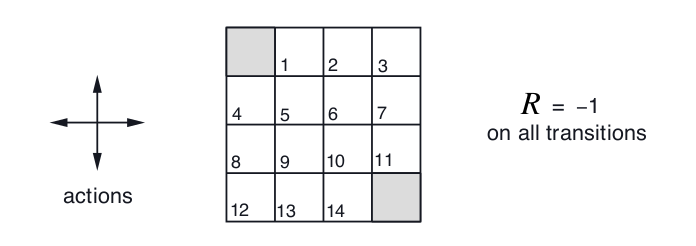
\includegraphics[width=1\textwidth]{Fig4-1.png}
\end{figure}

\one $S_t=14$에서 동서남북으로 움직일 수 있는데 동으로 움직일 경우만 $0$의 보상을 받고 나머지는 모두 $-1$의 보상을 받는다. 즉 
\begin{align*}
{\tt a=1}:\quad &\quad  \mathbb{E}_{\pi}(R_{t+1}|S_t=14)=\tt{P[14,1,1,13]{\cal R}[1]}\\
{\tt a=2}:\quad &\quad  \mathbb{E}_{\pi}(R_{t+1}|S_t=14)=\tt{P[14,1,1,13]{\cal R}[1]}\\
{\tt a=3}:\quad &\quad  \mathbb{E}_{\pi}(R_{t+1}|S_t=14)=\tt{P[14,1,1,13]{\cal R}[1]}\\
{\tt a=4}:\quad &\quad  \mathbb{E}_{\pi}(R_{t+1}|S_t=14)=\tt{P[14,1,1,13]{\cal R}[1]}\\
\end{align*}
이다. 
\[
\mathbb{E}_{\pi}(R_{t+1}|S_t=14)=\tt{polish[14,1]\left(\sum_{s'=1}^{|{\cal S}|}\sum_{r=1}^{|{\cal R}|}P[14,1,r,s']\times{\cal R}[r]\right)}
\]
\[
\mathbb{E}_{\pi}(R_{t+1}|S_t=14)=\tt{\sum_{a=1}^{4}}polish[14,a]P[s,a,r,s']
\]
\section{Polish Iteration}
\ck 특정 상태 $s \in {\cal S}$에 대하여 폴리쉬 $\pi^{(1)}(a|s)$가 좋은 폴리쉬인지 나쁜 폴리쉬인지 평가할 수 있다. 여기에서 숫자 1은 첫번째 폴리쉬라는 의미이다. 엔바이러먼트가 가진 테이블 $p(s',r|s,a)$과는 다르게 에이전트가 가진 테이블 $\pi(a|s)$는 업데이트가 된다. 즉 
\begin{align*}
\pi^{(1)}(a|s) \to \pi^{(2)}(a|s) \to .. 
\end{align*}
이런식으로 업데이트 하면서 더 좋은 테이블로 점점 수정해 나간다. 폴리쉬 $\pi^{(1)}(a|s)$ 이 좋은 폴리쉬인지 나쁜폴리쉬인지는 어떻게 알 수 있을까? 폴리쉬 $\pi'(a|s)$ 가 폴리쉬 $\pi(a|s)$ 보다 좋은 폴리쉬라고 주장하기 위해서는 (1) 각 정책에 대한 밸류펑션을 계산한뒤 즉 $v_{\pi}(s)$, $v_{\pi'}(s)$를 각각 계산한뒤에 (2) 모든 $s \in {\cal S}$에 대하여 아래가 성립함을 보이면된다. 
\begin{align*}
v_{\pi'}(s) \geq v_{\pi}(s)
\end{align*}
그러면 폴리쉬 $\pi'(a|s)$ 가 폴리쉬 $\pi(a|s)$ 보다 좋은 폴리쉬라고 생각할 수 있다. 

\ck 이런식으로 확장하면 더 이상 개선할 수 없는 폴리쉬가 있을텐데 \footnote{이게 존재함?? 이라고 생각할 수 있는데 존재한다고 한다.} 이를 \textbf{옵티멀폴리쉬(optimal policy)} 라고 하고 기호로는 $\pi^*(a|s)$ 와 같이 쓴다. 좀 더 엄밀하게는 가능한 모든 $\pi(a|s)$ 에 대하여 
\begin{align*}
\forall s \in {\cal S}: v_{\pi^*}(s) \geq v_{\pi}(s)
\end{align*}
이 성립할때 $\pi^*(a|s)$ 를 옵티멀폴리쉬라고 한다. 

\end{document}

